
\documentclass[12pt]{article}  % 此处选择 12 号字体

% 不需要填写年份,以当前电脑时间自动生成
\usepackage[2411457]{easymcm}  % 载入 EasyMCM 模板文件
\problem{E}  % 请在此处填写题号
\usepackage{mathptmx}  % Times 字体

\title{Property Insurance Sustainability, Real Estate Site Selection and Building Preservation Modeling Research Report}  % 标题

% 修改题头(默认为 MCM/ICM),使用以下命令(此处修改为 MCM)
%\renewcommand{\contest}{MCM}

% 文档开始
\begin{document}

% 此处填写摘要内容
\begin{abstract}
Against the backdrop of increasing global climate change, the frequency of extreme weather events has put unprecedented pressure on insurers, forcing them to seek balance in their underwriting strategies. In this paper, we use historical hazard data to predict the trend of future hazards, based on which we develop new underwriting strategies, and then switch the perspective to real estate developers and protectors of community landmarks, providing site selection suggestions and building preservation models for both of them, respectively.

First, a Vectors auto regression (VAR) model is used to characterize time series data for different types of extreme weather disasters in the same region and to predict the total number of disaster occurrences in the new year. The predicted results for each region were ALABAMA 135, LOUISIANA 1921, NEW YORK 1082, etc. The relationship between the number of disaster occurrences and the amount of natural disaster losses is derived by using fitting, and the distribution of predicted property loss rates is obtained by fitting the total assets with return on assets and GDP.

Second, in the process of determining the underwriting strategy, the expected utility maximization is used to describe the customer behavior, and from the financial statements, it is concluded that "the profit of the insurance company comes from the difference between the premiums and the amount of claims and the investment income", and then the relationship between the proportion of premiums in each state and the stochastic distribution of the total profit of the insurance company is calculated. A computational model of the optimal underwriting strategy is given by translating the operational needs of the insurance company into requirements that characterize the stochastic distribution of total profits.

Then, in the community and real estate siting model, the effects of population, age structure, and total real estate on real estate risk were combined using correlation analysis and normalized scoring, and the benefits of insurance companies in avoiding natural disaster risks were assessed using the insurance company underwriting strategies for each region in the previous model.

Finally, the building preservation model quantifies the loss of cultural value, relocation costs, and restoration costs of the buildings using a fuzzy comprehensive evaluation method. The magnitude of relocation costs and in-situ preservation costs were evaluated to determine specific preservation strategies. We assumed that the effect of physical loss of a building on cultural value decreases with the age of the building, and the model was transformed into a comparison of the discounted value of extreme weather loss in terms of cultural value and relocation costs. We also use the Willis Tower in Chicago as an example to get the conclusion that the building does not need to be relocated in the next 20 years.


\end{abstract}



\maketitle  % 生成 Summary Sheet
\tableofcontents  % 生成目录


% 正文开始
\section{Introduction}
\subsection{Problem Background}
As global climate change intensifies, the frequency and intensity of extreme weather events continues to rise, posing unprecedented challenges to the property insurance industry. In recent years, property owners and insurers around the world have experienced significant financial losses from natural disasters such as floods, hurricanes, cyclones, droughts and wildfires. According to the Boston Consulting Group, claims for natural disasters in 2022 are 115 percent higher than the 30-year average, a trend that signals higher pressure on insurers to pay out in the future. Meanwhile, data from Munich RE shows that weather disaster losses suffered by the U.S. dominate global natural catastrophe losses in 2021. These figures not only reveal a widening insurance coverage gap, but also reflect a dual crisis in insurers' profitability and homeowners' affordability.

\begin{figure}[htbp]
\centering
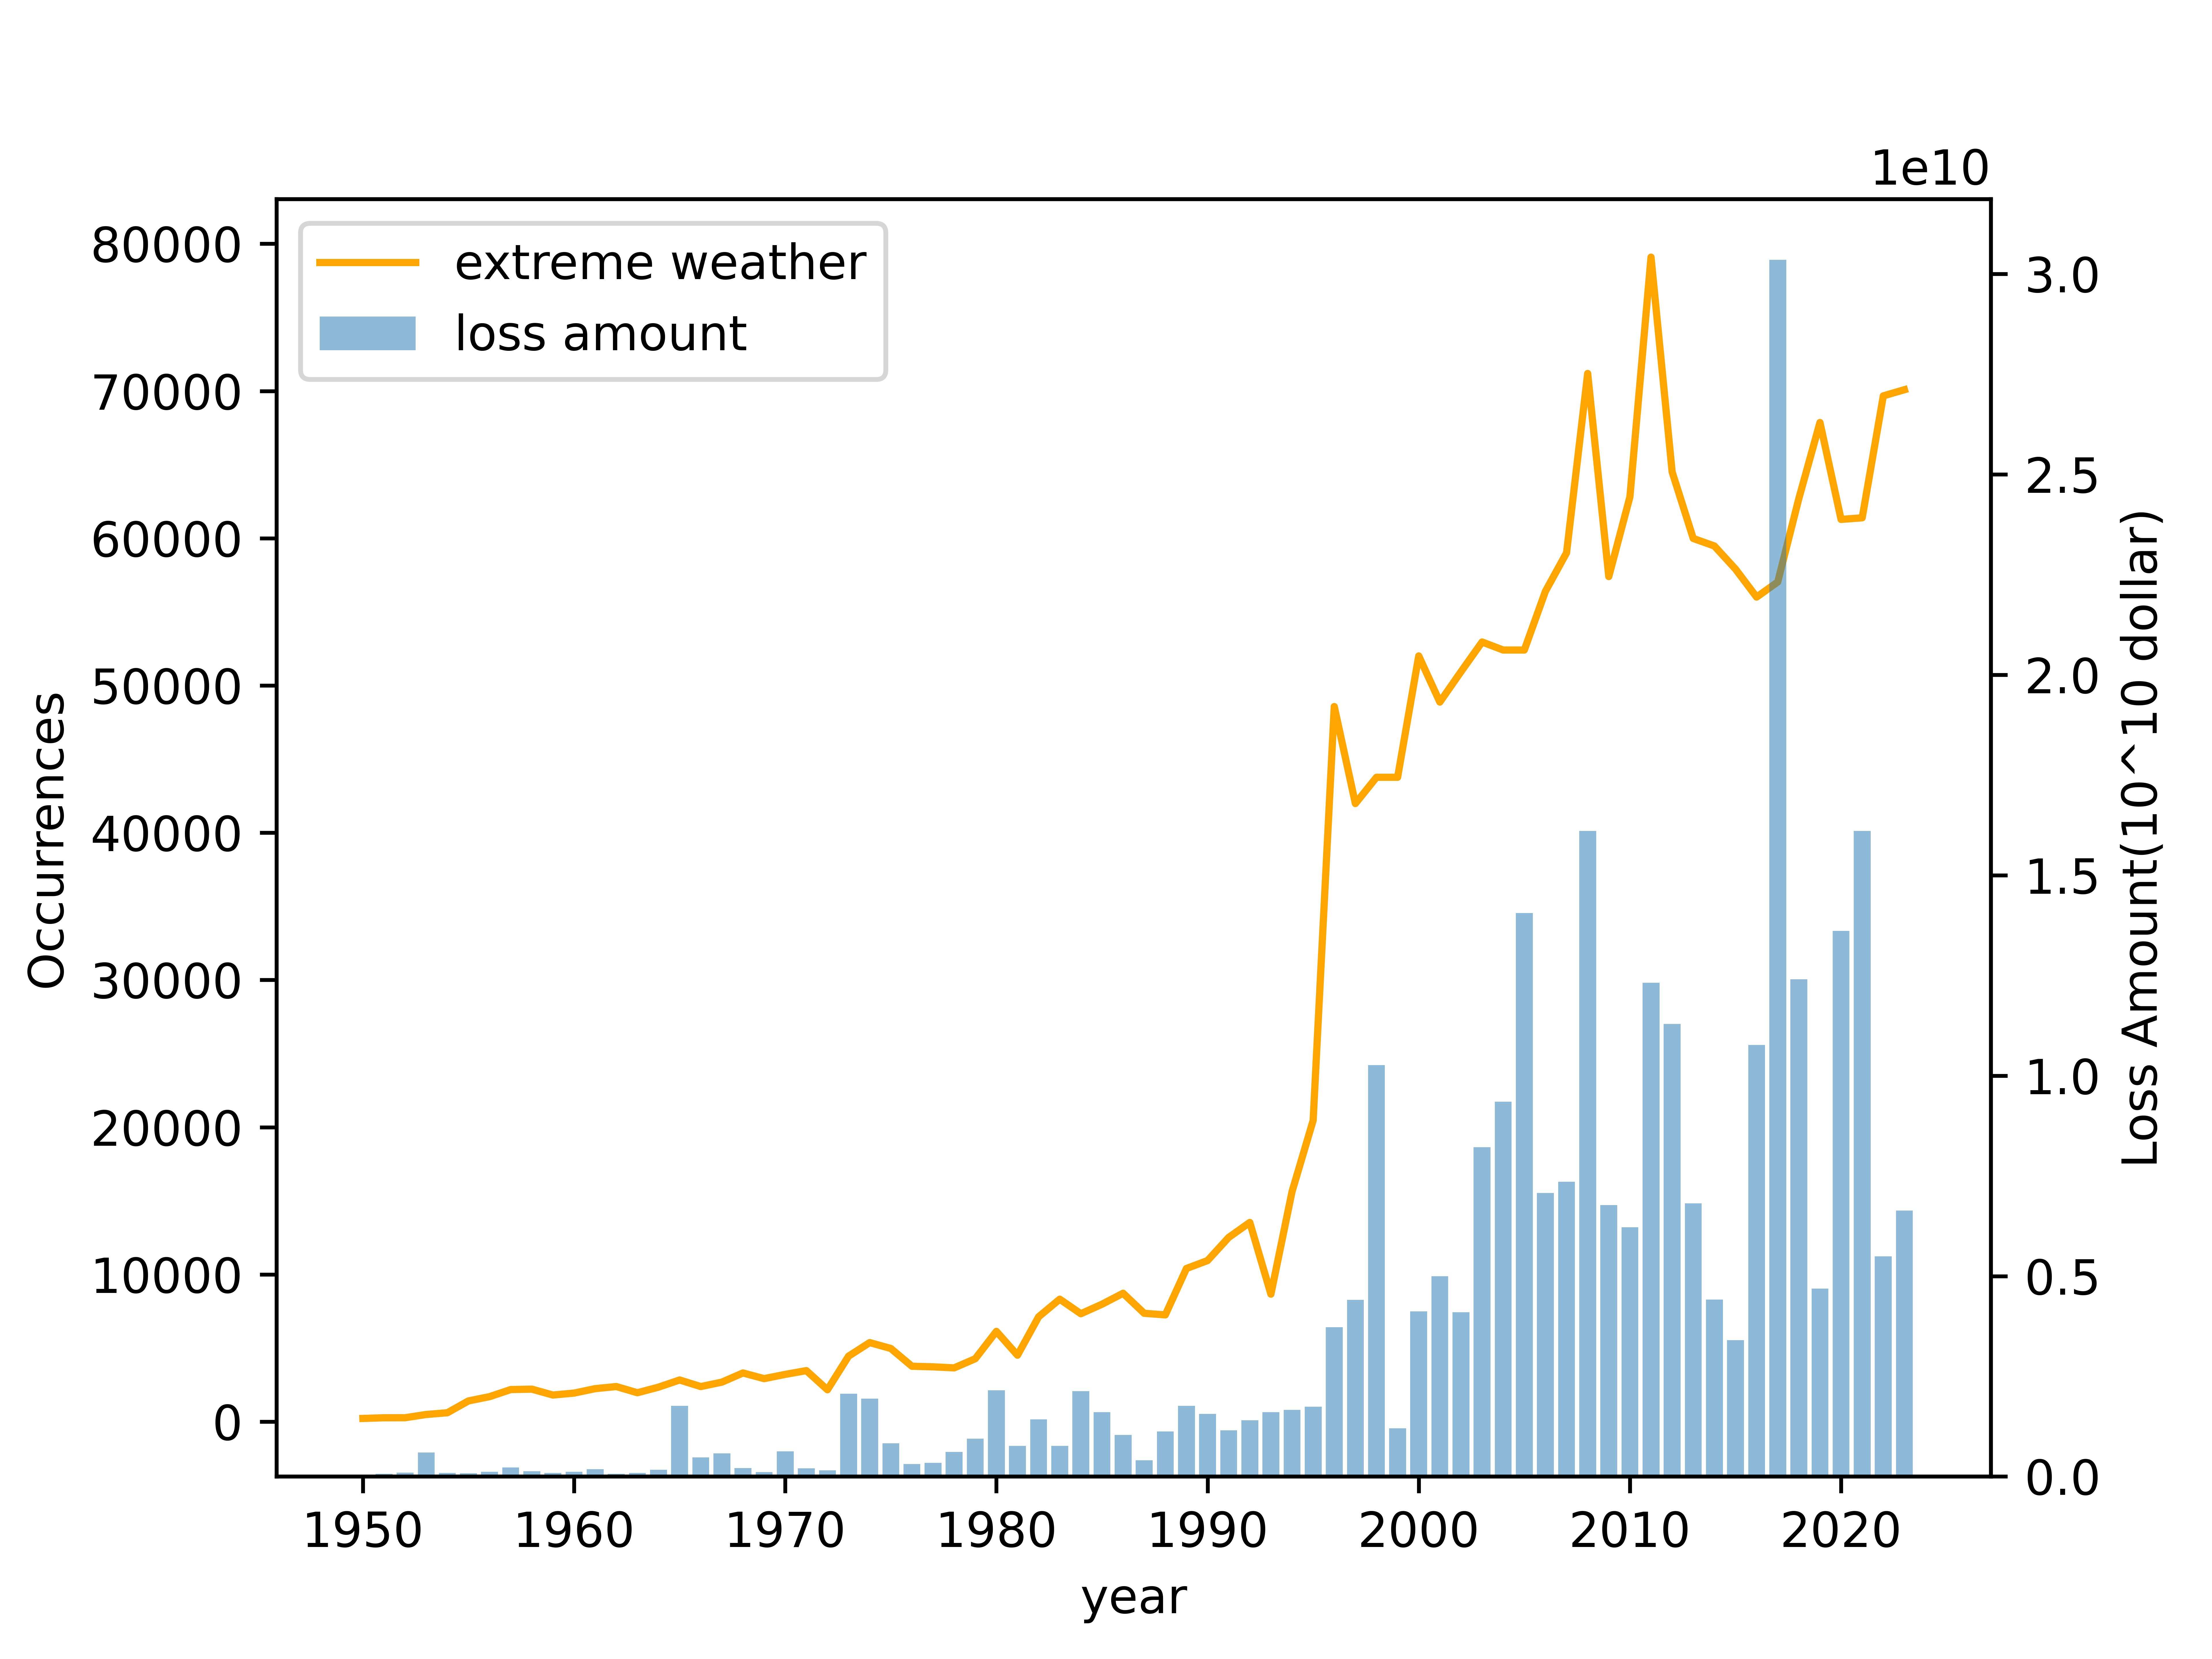
\includegraphics[width=.7\textwidth]{img/img05.png}
\caption{Natural Disasters and Losses}
\end{figure}

Against this backdrop, the sustainability of property insurance has become a pressing issue. How insurers can strike a balance in their underwriting strategies to ensure their own long-term health while providing necessary protection for property owners has become a key issue. Additionally, communities and real estate developers must consider changes in insurance models when planning and building to ensure resilience and sustainability of new properties. In some cases, insurance models may recommend that certain areas not be covered by property insurance, which will force community leaders to make difficult decisions when it comes to preserving culturally, historically, or community-significant properties.


\subsection{Literature Review}
Against the backdrop of extreme weather events, insurers urgently need to update their pricing strategies. The report Private Flood Insurance and the National Flood Insurance Program highlights the efforts of the U.S. National Flood Insurance Program (NFIP) to address climate change risks, as well as private insurers' interest in the flood insurance market, driven by advances in risk analytics and data technology growing. However, challenges in the legislative and regulatory framework require insurers to exercise caution when developing their strategies.

The variability in consumer protection is having an impact on the stability of the private insurance market and consumer trust, and insurers need to ensure the accuracy of their risk assessments while offering flexible and low-cost insurance products. This requires not only historical loss data and flood map information, but also consideration of the impact of changes in the natural catastrophe insurance market on other markets.

Merton's (1973) Interperiod Capital Asset Pricing Model (ICAPM) provides insurers with a theoretical basis for understanding the dynamics of asset prices, while Markowitz's (1952) portfolio theory guides the search for a balance between risk and return.Fama and MacBeth's (1973) empirical study of the CRRA utility function reveals investors' risk aversion, which is critical for insurers to understand market demand.Bakkensen and Barrage's (2017) study demonstrates the impact of flood risk beliefs on property prices through correlation analysis, while Kapphan, Calanca, and Holzkaemper's (2012) fuzzy valuation methodology offers a new perspective on responding to climate change provides a new perspective.

These studies provide theoretical support and practical guidance for insurers as they update their pricing strategies, helping them find a balance between risk management, market interactions, and consumer demand. Policymakers and insurers should continue to explore ways to promote market participation and ensure the affordability and appropriateness of insurance coverage, taking into account the recommendations in Fifty Years of U.S. Natural Disaster Insurance Policy, in order to achieve long-term stability and sustainability in the insurance market. Future research should further explore how these factors can be synthesized to provide insurers with more comprehensive strategic guidance.

\subsection{Our work}
We did all this to get the job done. Here is a schematic of the modeling framework.

\begin{figure}[htbp]
\centering
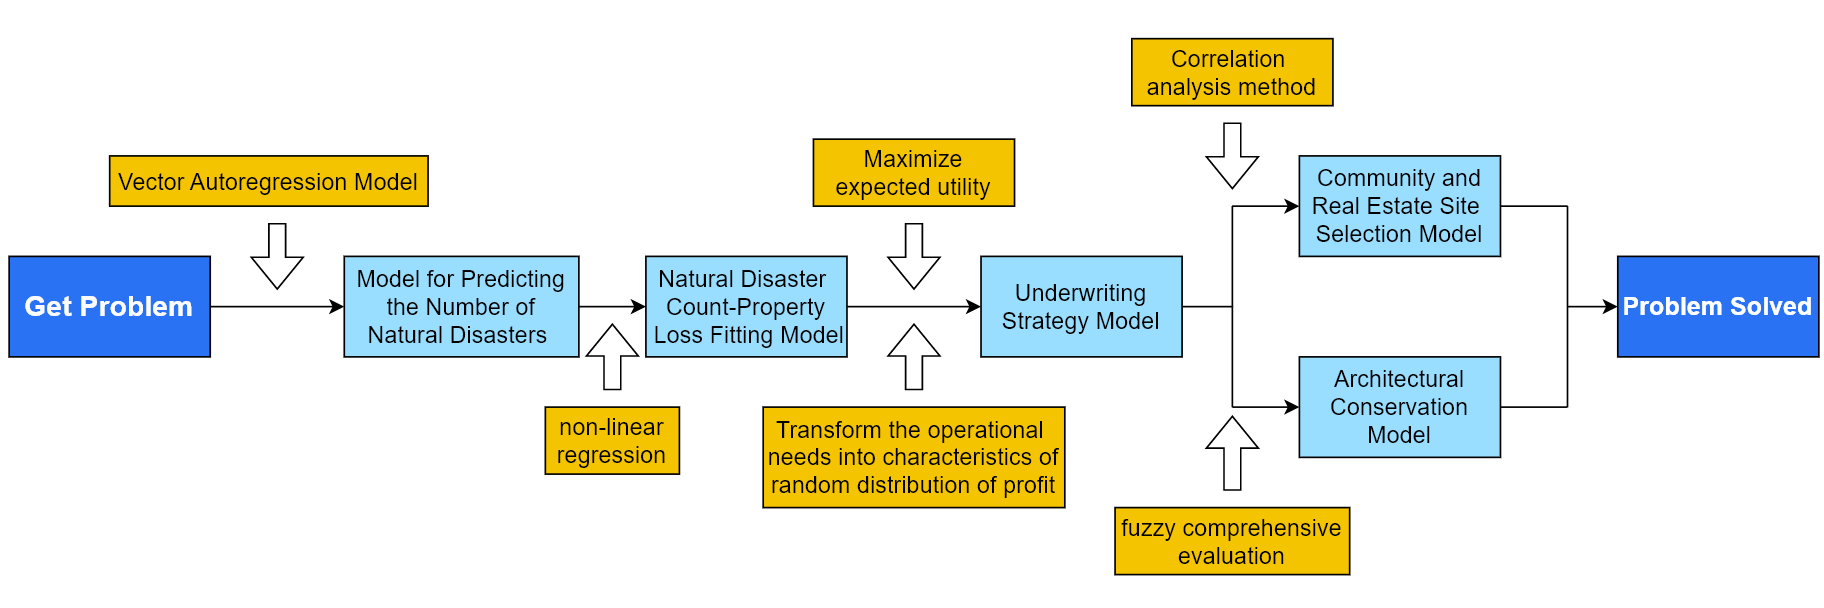
\includegraphics[width=0.9\textwidth]{img/img08.png}
\caption{Schematic Diagram of the Model Framework}
\end{figure}

\clearpage

\begin{enumerate}[\bfseries 1.]
    \item In formulating the underwriting strategy, we first surveyed and counted the historical disasters in the area we wanted to examine whether and with what strategy to underwrite, selected the top 10 natural disasters, and analyzed them in a time series to predict the number of occurrences of each disaster in the future. Since it was assumed that each natural disaster would cause a certain amount of damage when it occurs, the number of occurrences of each natural disaster for each year in the region was totaled. Next, the amount of historical natural disaster losses in the region is examined, fitted to the historical number of natural disaster occurrences, and losses due to future natural disaster occurrences are projected. In addition, the total economic output of the region was estimated by taking into account the historical GDP of the region, and the premiums charged were calculated with reference to the losses predicted above as an underwriting strategy.
    \item In constructing the community and real estate location model, we examine whether an area is suitable for real estate development by taking into account many factors in the area. From the region's population, age structure, real estate total quantified by the real estate demand and future development potential index, from the insurance strategy, the number of natural disasters quantified by the real estate risk, and finally by the demand and development potential, risk index quantitative real estate location index, the index is a relative measure, the larger the value indicates that the more suitable for real estate location.
    \item On the community preservation model, we consider the actual wear and tear of the building, cultural depreciation, relocation costs, repair costs, etc., and use the fuzzy comprehensive evaluation method to construct an evaluation model and evaluation criteria, quantify the individual costs and calculate the minimum value of the cumulative costs, and make a conclusion on the community preservation strategy.
\end{enumerate}


\section{Preparation of the Models}
\subsection{Assumptions}
In developing our underwriting strategy, we have made the following assumptions.
\begin{itemize}
    \item Insurance companies sell natural disaster insurance, i.e., losses and claims are only considered to be caused by natural disasters.
    \item There are up to 10 natural disasters that cause significant economic losses in a region, i.e., in order to make the predictions of the time series analysis more reliable and to reduce the possibility of non-convergence, the economic losses in each region are only caused by the 10 natural disasters that occur most frequently in the region.
    \item In order to simplify the model, it is assumed that the loss caused by each type of natural disaster is certain and consistent for each occurrence.
    \item In the analysis of the insurance strategy, it is assumed that the insurance period is fixed at 1 year, which simplifies the game between the insurance company and the policyholder about the insurance period.
    \item The Gross Domestic Product (GDP) of a region can be used to estimate the total economic output, and it is assumed that the total economic output will not change in the future insurance cycle, i.e., within 1 year.
    \item The logarithm of the amount of money lost in a particular natural disaster is normally distributed.
    \item The value of $\ln lpr$ in natural disasters in a given area is normally distributed.
    \item Insurance companies generally choose a low-risk, long-duration, profit-margin-certain investment strategy, so the return on an insurance company's investment is assumed to be an exogenous variable.
    \item Customers in different states have the same distribution of risk aversion coefficients $\theta$.
    \item Assume that the insurance company's existing strategy only considers profit maximization under complete risk diversification.
\end{itemize}

In the community and real estate site selection model, we have the following assumptions.
\begin{itemize}
    \item The level of urbanization development is equal to the urbanization rate.
    \item The function of the level of urbanization on real estate development indicators is trigonometric.
    \item The urban consumption index is equal to the price index of personal consumption expenditures, i.e. real consumer expenditures, corrected by the regional price parity (RPP) method. Corrected for the impact of different regional prices on the price index of personal consumption expenditure.
    \item When the real estate company chooses not to insure, the insurance company does not help the real estate company's risk-taking by setting the score to 0. And this will be reflected in the decision outcome by making the correction.
\end{itemize}

The following assumptions were made when modeling building preservation.
\begin{itemize}
    \item The value of the building is lost only due to weather conditions.
    \item The building loses value at a certain rate each year.
    \item The building costs a certain amount of money to relocate, and it is assumed that the relocation is to a place with ideal weather conditions, so that the cost of repairs can be ignored for a short period of time (20 years).
    \item Loss of cultural value tends to 0 (<1\%) after 100 years of building construction.
\end{itemize}


\subsection{Notations}
In developing our coverage strategy, we used the following notations.

\begin{longtable}{ c p{28em} }
\caption{Notations for Coverage Strategy}
\label{tb:longtable}\\
\toprule
\multicolumn{1}{m{3cm}}{\centering Symbol}
	&\multicolumn{1}{m{11cm}}{\centering Definition}\\
\midrule
$st$ & Aggregation of all districts for which an enrollment strategy is to be developed \\
$st[x]$ & $x$th region where an enrollment strategy is to be developed \\
$dis$ & Aggregation of natural disasters counted \\
$dis[x]$ & $x$th natural disaster counted \\
$dis_{x,t}$ & Vector of the number of occurrences in year $t$ of the 10 natural hazards with the highest total number of occurrences in $x$th region \\
$t$ & year \\
$dis\_sum_{x,t}$ & Sum of the number of occurrences in year $t$ of the 10 natural disasters with the highest total number of occurrences in $x$th region \\
$dp_{x,t}$ & Vector of the amount of losses due to natural disasters by region in year t \\
$nao$ & Beginning net assets of an area, also total assets \\
$nac$ & Closing net assets of an area \\
$nagr$ & Growth rate of net assets in a region \\
$lpr$ & Projected rate of property damage due to natural disasters in an area in the coming year \\
$\Pi$ & Premiums offered by insurance companies for a given area as a percentage of the insured amount \\
$\theta$ & Relative risk aversion coefficients in utility functions \\
$Inc$ & Profits of insurance companies \\
$Inv$ & Income from investment business of insurance companies \\
$Rev$ & Premium income from insurance companies \\
$OE$ & Operating expenses of insurance companies \\
$Claim$ & Amount paid by the insurance company \\
$Prop$ & The amount of property insured as a percentage of total assets in a region \\
$Inc_{invest}$ & I.e. $Inv$, meaning the part of income that comes from investment \\
\bottomrule
\end{longtable}

In the Community and Real Estate Site Selection Model, we use the following notations.

\begin{longtable}{ c p{28em} }
\caption{Notations for Real Estate Site Selection}
\label{tb:longtable}\\
\toprule
\multicolumn{1}{m{3cm}}{\centering Symbol}
	&\multicolumn{1}{m{11cm}}{\centering Definition}\\
\midrule
$rei_j$ & Indicators of real estate development in region j \\
$U_j$ & Level of urbanization development in region j \\
$C_j$ & Urban consumption index for region j \\
$GDPg_j$ & GDP growth rate in Region j \\
$\Pi_{i,j}$ & Psychological price of premium ratio of entity i to region j \\
$D_{i,j}$ & Results of entity i's decision on whether or not to insure region j \\
$I_{i,j}$ & Post-decision benefits of entity i in region j \\
$score_{i,j}$ & Entity i's rating of whether or not real estate development is taking place in region j \\
$point_{i,j}$ & Normalized score of entity i on whether or not real estate development is taking place in region j \\

\bottomrule
\end{longtable}


On the architectural conservation model, we use the following notations \ref{notation3}.

\begin{table}[!htbp]
\begin{center}
\caption{Notations for Architectural Conservation}
\begin{tabular}{cl}
	\toprule
	\multicolumn{1}{m{3cm}}{\centering Symbol}
	&\multicolumn{1}{m{12cm}}{\centering Definition}\\
	\midrule
	$t$&Number of years that have elapsed since the building was constructed\\
	$C_t$&Loss of cultural value in year $t$ after construction\\
	$al_t$ &Losses due to weather in year $t$ after construction\\
        $r$ &Discount rate for cultural values\\
        $mt_{t_0}$ &Maintenance costs from completion to $t_0$ years after completion\\
        $mc$ &Transfer of building costs\\
        $mtc_t$ &Loss of cultural value of buildings constructed or maintained for $t$ years\\
        $lpr$ &Projected property loss rate for an area for the coming year\\
        $rl$ &Cost of relocation of buildings\\
        $tv$ &Total value of buildings\\
        $tl$ &Total costs due to construction over the next 20 years\\
	\bottomrule
\end{tabular}\label{notation3}
\end{center}
\end{table}



\section{The Models}
\subsection{Model for Predicting the Number of Natural Disasters}
\subsubsection{Model Building}
For region $x$, the vector of occurrences of the 10 natural hazards with the highest total number of occurrences in year $t$ is as follow.
\begin{align*}
dis_{x,t}=(dis_{1,x,t},dis_{2,x,t},...,dis_{10,x,t})'
\end{align*}

Since all the discussion is now based on the $x$th region, we start by omitting $x$ and simplifying the expression.
\begin{align*}
dis_{t}=(dis_{1t},dis_{2t},...,dis_{10t})'
\end{align*}
Consider using a fitting and prediction model with a lag order of 5, where $\epsilon_t$ is the error, which should converge to 0 as much as possible in the fit.
\begin{align*}
dis_{t}=\phi_{1}dis_{t-1}+\phi_{2}dis_{t-2}+...\phi_{5}dis_{t-5}+\epsilon_{t}
\end{align*}
Assuming that the starting and ending years of all the data surveyed are $t_0$, $t_1$, then one can obtain the system of equations.
\begin{align*}
\begin{cases}
dis_{t_0+5}=\phi_{1}dis_{t_0+4}+\phi_{2}dis_{t_0+3}+...\phi_{5}dis_{t_0}+\epsilon_{t_0+5}
\\
dis_{t_0+6}=\phi_{1}dis_{t_0+5}+\phi_{2}dis_{t_0+4}+...\phi_{5}dis_{t_0+1}+\epsilon_{t_0+6}
\\
...
\\
dis_{t_1}=\phi_{1}dis_{t_1-1}+\phi_{2}dis_{t_1-2}+...\phi_{5}dis_{t_1-5}+\epsilon_{t_1}
\end{cases} 
\end{align*}
The goal is to minimize $\sum\limits_{i=t_0+5}^{t_1} \epsilon_i$. Then the coefficients $\phi_1$, $\phi_2$, $\phi_3$, $\phi_4$, $\phi_5$, can be solved by methods such as least squares.
Bringing the coefficients into the following equation.
\begin{align*}
dis_{t_1+1}=\phi_{1}dis_{t_1}+\phi_{2}dis_{t_1-1}+...\phi_{5}dis_{t_1-4}
\end{align*}
Get the predicted value of $dis_{t1}$.

\subsubsection{Model Utilization}

The following is an analysis of the United States and surrounding areas as an example.
Approximately 1.79 million natural disaster records were found for the years 1950-2023 for the United States and surrounding areas. The form of the data is given below:


\begin{table}[!ht]
    \centering
    \caption{Data Format}
    \begin{tabular}{|l|l|l|l|l|l|}
    \hline
        year & month & day & region & type & damage\_property \\ \hline
        1955 & 6 & 22 & NEW JERSEY & Thunderstorm Wind & 0 \\ \hline
        2019 & 7 & 3 & INDIANA & Flash Flood & 35000 \\ \hline
        2011 & 4 & 5 & NORTH CAROLINA & Thunderstorm Wind & 2000 \\ \hline
        1994 & 6 & 24 & NEBRASKA & Hail & 500000 \\ \hline
    \end{tabular}
\end{table}

A total of 70 disasters recorded in the data were counted, or $st$. The regions were divided into 68, or $dis$.

The data is divided into regions and the number of occurrences of each type of disaster is counted separately for each region in each year. Taking $st[8]$, i.e., CALIFORNIA, as an example, the top 10 natural disasters are: Dense Fog, Drought, Flash Flood, Flood, Heavy Rain, Heavy Snow, High Wind, Strong Wind, Wildfire, and Winter Storm. ...Remember these 10 natural disasters as $dis[1]$, $dis[2]$, ... , $dis[10]$.

Then we can statistically get $dis_{8,1950}$ to $dis_{8,2023}$


\begin{table}[!ht]
    \centering
    \begin{tabular}{|c|c|}
    \hline
    Variable & Value\\ \hline
        $dis_{8,1950}$ & $(0,0,0,0,0,0,0,0,0,0)'$  \\ \hline
        ... & ...  \\ \hline
        $dis_{8,2022}$ & $(155,606,172,164,125,155,473,129,42,50)'$  \\ \hline
        $dis_{8,2023}$ & $(42,19,230,749,70,282,471,191,21,71)'$  \\ \hline
    \end{tabular}
    \caption{\label{demo-table}Results}
\end{table}

The predicted value of $dis_{8,2024}$ is obtained using the above model as

$(123,179,400,-212,227,264,44,179,-28,128)'$

Therefore, $dis\_sum_{8,2024}=1307$ is used as the predicted number of disasters for the CALIFORNIA area.

Similarly, the remaining 67 districts were predicted and the following results were obtained. The results are as follows.


\begin{table}[!ht]
    \centering
    \begin{tabular}{|l|l|l|l|l|l|}
    \hline
        ALABAMA & 135 & IOWA & 1263 & NEW YORK & 1082 \\ \hline
        ALASKA & 228 & KANSAS & 1803 & NORTH CAROLINA & 816 \\ \hline
        AMERICAN SAMOA & 15 & KENTUCKY & 1176 & NORTH DAKOTA & 598 \\ \hline
        ARIZONA & 742 & LAKE ERIE & 46 & OHIO & 607 \\ \hline
        ARKANSAS & 1082 & LAKE HURON & 7 & OKLAHOMA & 2548 \\ \hline
        ATLANTIC NORTH & 393 & LAKE MICHIGAN & 45 & OREGON & 222 \\ \hline
        ATLANTIC SOUTH & 294 & LAKE ONTARIO & 6 & PENNSYLVANIA & 764 \\ \hline
        CALIFORNIA & 1307 & LAKE ST CLAIR & 8 & PUERTO RICO & 173 \\ \hline
        COLORADO & 1468 & LAKE SUPERIOR & 51 & RHODE ISLAND & 55 \\ \hline
        CONNECTICUT & 118 & LOUISIANA & 1921 & SOUTH CAROLINA & 523 \\ \hline
        ... & ... & ... & ... & ... & ... \\ \hline
    \end{tabular}
    \caption{\label{demo-table}Results of All Region}
\end{table}

\begin{figure}[htbp]
\centering
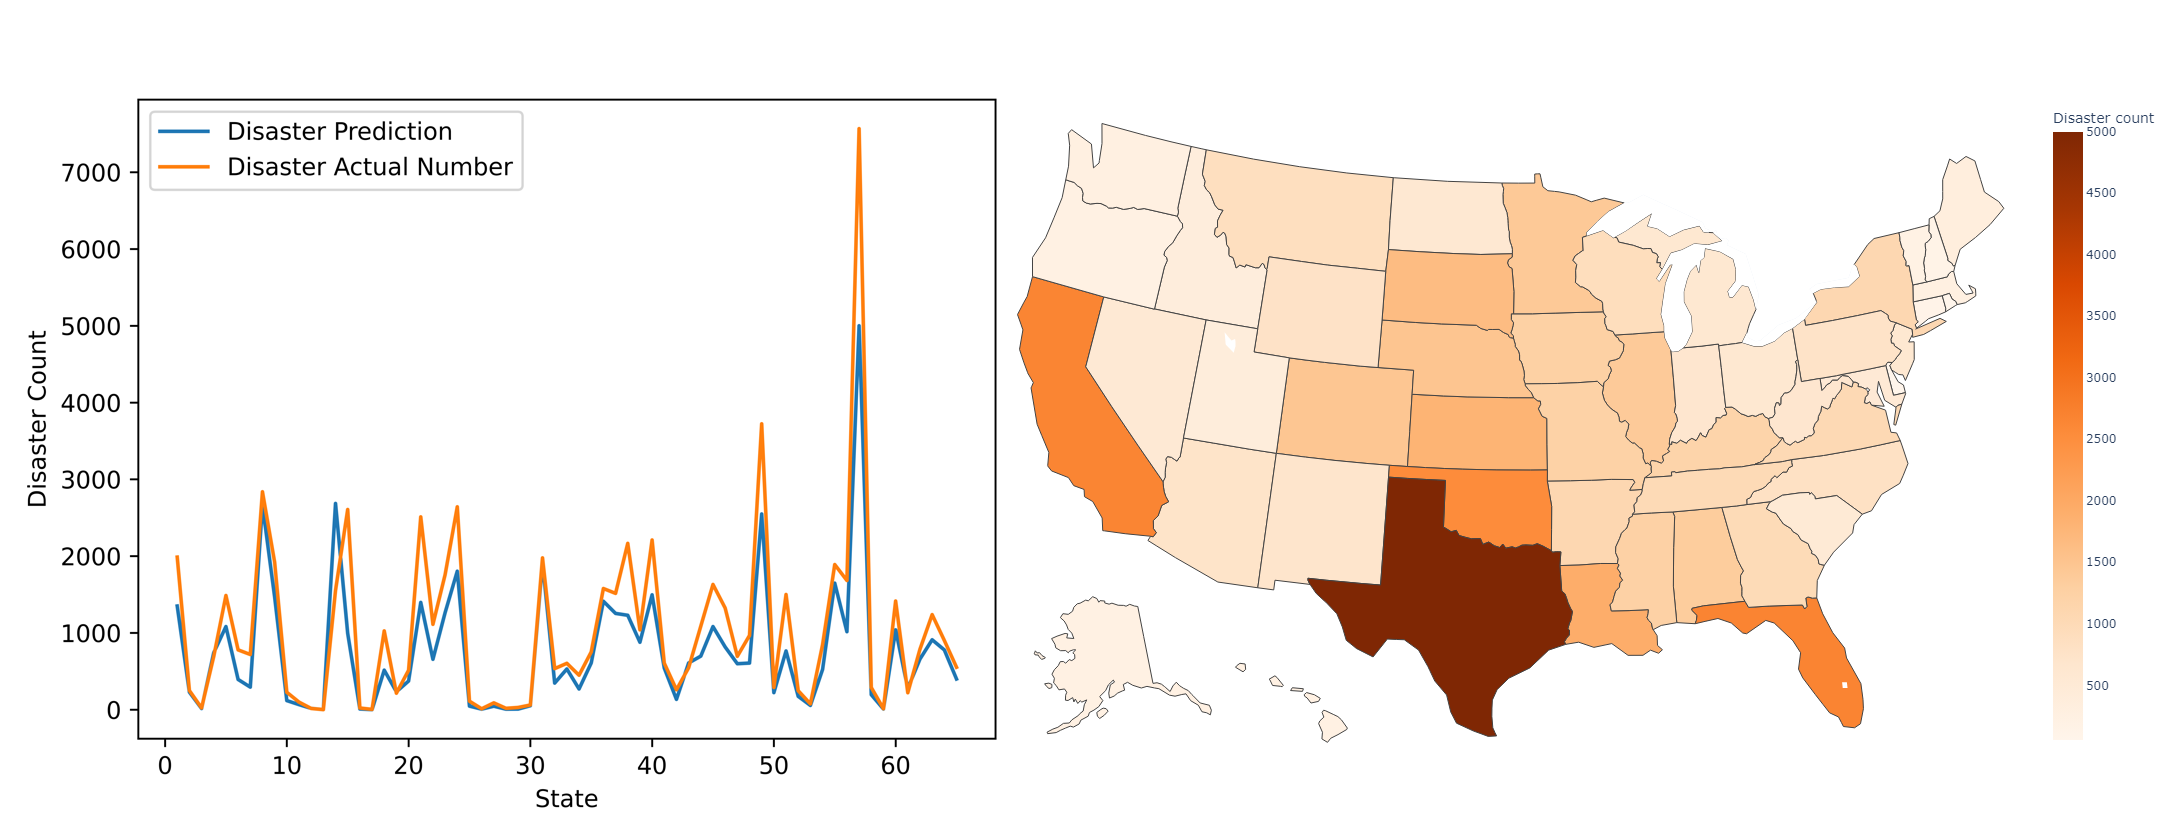
\includegraphics[width=1\textwidth]{img/img02.png}
\caption{Visual of Results: The horizontal coordinates of the map on the left indicate the number of districts}
\end{figure}


\subsection{Natural Disaster Count-Property Loss Fitting Model}
\subsubsection{Model Building}
Since it is assumed that the logarithmic value of the rate of property damage in natural disasters in a given area is normally distributed, the number of natural disasters and property damage show a power function relationship, i.e.
\begin{align*}
    y=ax^b
\end{align*}
where $y$ is property damage and $x$ is the number of natural disasters.

To make it linear, taking logarithms of the equation yields.
\begin{align*}
    \ln y=b\ln x +  \ln a
\end{align*}
Bringing all $(dis\_sum_{x,t},dp_{x,t})$ as a dataset yields
\begin{align*}
    \begin{bmatrix}
\ln x_1 & 1 \\
\ln x_2 & 1 \\
... \\
\ln x_n & 1 
\end{bmatrix}
\begin{bmatrix}
b \\
\ln a
\end{bmatrix}
=
\begin{bmatrix}
\ln y_1 \\
\ln y_2 \\
... \\
\ln y_n
\end{bmatrix},
\quad where \quad 
X=
\begin{bmatrix}
\ln x_1 & 1 \\
\ln x_2 & 1 \\
... \\
\ln x_n & 1 
\end{bmatrix},
Y=\begin{bmatrix}
\ln y_1 \\
\ln y_2 \\
... \\
\ln y_n
\end{bmatrix}
\end{align*}
The least squares equation is
\begin{align*}
    X'X
\begin{bmatrix}
\widehat{b}  \\
\ln \widehat{a} 
\end{bmatrix}
=
X'Y
\end{align*}
From there, the $\widehat{a}$ , $\widehat{b}$ can be solved, and the process of linear regression is complete. Using the regression equation, combined with the number of natural disasters in each area predicted by the previous model, property damage in each area can be predicted.


\subsubsection{Model Utilization}
The previous model's example of the U.S. and surrounding regions was then fitted.

Each region was fitted and predicted separately, and all years of data for a region were summarized for a total of 74 data points. The outliers in the number of natural hazards are too large probably due to errors in documentation or non-convergence of the predictions, and the data points with a natural hazard number of 0 are most likely due to missing data records too early in the year, so these were cleaned and excluded, and an exponential regression was performed on the remaining data points, which yielded the following results.


\begin{table}[!ht]
    \centering
    \begin{tabular}{|l|l|l|}
    \hline
        area & a & b \\ \hline
        ALABAMA & 74184.06546 & 0.904823951 \\ \hline
        ALASKA & 188955.6479 & 0.692844191 \\ \hline
        AMERICAN SAMOA & 77394461956 & -3.791897753 \\ \hline
        ARIZONA & 344.7640509 & 1.779958561 \\ \hline
        ... & ... & ... \\ \hline
    \end{tabular}
    \caption{\label{demo-table}Coefficient Examples}
\end{table}

\clearpage

\begin{figure}[htbp]
\centering
\includegraphics[width=.6\textwidth]{img/img03.png}
\caption{Some Regions' Fitted Curve}
\end{figure}


Using the fitted exponential curves to predict property damage in each area, we get the final result.

\begin{table}[!ht]
    \centering
    \begin{tabular}{|l|l|l|l|}
    \hline
        ALABAMA & 46875935.53 & MONTANA & 1853809.502 \\ \hline
        ALASKA & 5568615.404 & NEBRASKA & 44247581.83 \\ \hline
        ARIZONA & 34321842.94 & NEVADA & 73841023.57 \\ \hline
        ARKANSAS & 38015766.9 & NEW HAMPSHIRE & 730582.1857 \\ \hline
        CALIFORNIA & 9055952380 & NEW JERSEY & 6270702.012 \\ \hline
        ... & ... & ... & ... \\ \hline
    \end{tabular}
    \caption{\label{demo-table}Projections of Property Damage by Region}
\end{table}

The results were subjected to error analysis for each region, calculated $RSS$, $TSS$ and $R^2$, the 10 regions with the highest correlation coefficients had correlation coefficients greater than 0.6, indicating a more accurate fit using the index model.

\begin{figure}[htbp]
\centering
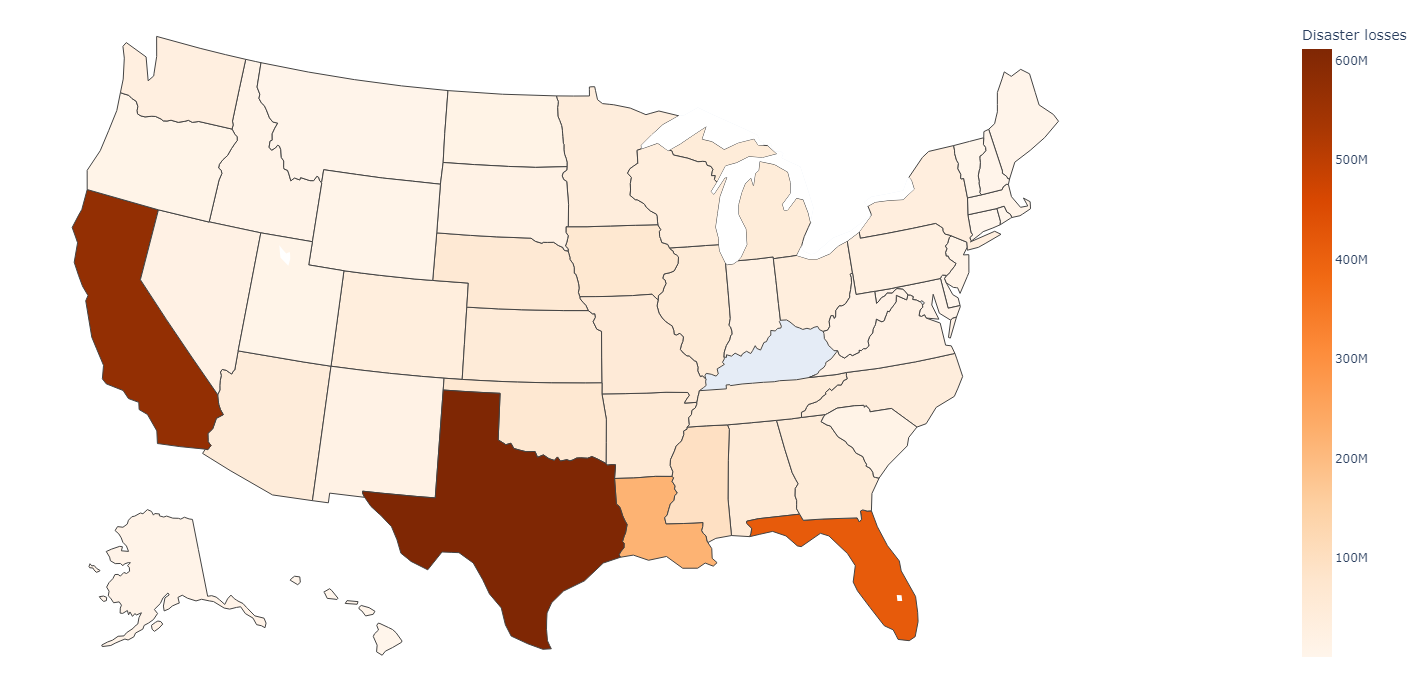
\includegraphics[width=.62\textwidth]{img/img04.png}
\caption{Visual Map of Results}
\end{figure}

\clearpage

\subsection{Underwriting Strategy Model}
\subsubsection{Determination of Property Damage}
Without loss of generality, we assume that all policies have a term of 1 year and that the payout is the portion of the loss that replenishes the insured property. When the above model predicts the amount of loss in the coming year, the most explanatory order is 5 if we use the AIC (Akaike Information Criterion) as a lag order judgment criterion; we choose a 4th order lag, which introduces more sensitivity to the most recent year's weather extremes for the underwriting strategy.

Since in the underwriting strategy we assume that customers are relatively risk averse invariant, i.e., have a CRRA utility function, and that the proportion of acceptable premiums (premiums as a percentage of insured amount) does not vary with the insured amount, the amount of the loss as a percentage of the stock of assets is a more direct influence. The stock of assets for each region is calculated below.

From the net asset growth rate formula as below.
\begin{align*}
    nagr= \frac{nac-nao}{nao} \times 100\%
\end{align*}
It can be rolled out:
\begin{align*}
    nao= \frac{nac}{1+nagr}
\end{align*}

From this, the $nao$ for each region can be calculated, and taking up the property losses predicted by the above model for each region, the distribution of the predicted property loss rate $lpr$ for each region can be obtained.

\subsubsection{Relationship between Premium Ratios and Utility Functions}
Since it is assumed that the values of $\ln lpr$ in natural disasters in each state are normally distributed, i.e.
\begin{align*}
    \ln (lpr) \sim N(a,b^2)
\end{align*}
There are some regions for example according to the calculation method above.


\begin{table}[!ht]
    \centering
    \begin{tabular}{|l|l|l|}
    \hline
        Region & $a$ & $b^2$ \\ \hline
        ALABAMA & -10.9740088 & 2.113475458 \\ \hline
        ALASKA & -11.37597287 & 1.292062183 \\ \hline
        ARIZONA & -11.64055518 & 5.492655469 \\ \hline
        ARKANSAS & -10.3579003 & 2.453277449 \\ \hline
    \end{tabular}
    \caption{Parameter of Normal Distribution of Some Regions}
\end{table}

The CRRA utility function $U$ uses
\begin{align*}
    U( \widetilde{Y} )= \frac{\widetilde{Y}^{1-\theta}}{1-\theta}
\end{align*}
Where $\theta$ is the relative risk aversion coefficient, which is only relevant for the client group.

Then we can assume that $\theta  \sim N( \overline{\theta},\sigma^2_{\theta} )$. $\theta_i$ denotes the relative risk aversion coefficient of the $i$th customer. Noting that $Y_{i,0}$ is the value of the property that the $i$th customer wants to insure, and $Y_{i,1}$ is the value of the property after 1 year if the $i$th customer is not insured, then there are
\begin{align*}
    Y_{i,1}=Y_{i,0}(1-lpr)
\end{align*}

It is assumed that customers choose whether or not to be insured according to expected utility maximization, $E(U(Y_{i,1}))$ is the expected utility of not being insured, and $E(U(Y_{i,0}-r_{i}))$ is the expected utility of being insured. where $r_i$ is the premium charged to the $i$th customer, $Y_{i,1}$ is a random variable, and both $Y_{i,0}$ and $r_i$ are fixed values.

Customers will choose to purchase insurance only when 
\begin{align*}
    E(U(Y_{i,1}))<E(U(Y_{i,0}-r_{i}))=U(Y_{i,0}-r_{i})
\end{align*}

Then the maximum value of the premium that can be charged to the $i$th customer is
\begin{align*}
    r_i^*=- \frac{U''}{U'} \frac{Var[Y_{i,0}(1-lpr)]}{2} 
=- \frac{U''}{U'} \frac{Var(Y_{i,0}lpr)}{2} 
= \frac{\theta_i}{Y_{i,0}} \frac{1}{2}Y_{i,0}^2e^{2a}(e^{2b^2}-e^{b^2})
\end{align*}
It can be obtained that the upper limit of the percentage of premium that the $i$th customer can accept is
\begin{align*}
    \Pi_i^*=\frac{r^*_i}{Y_{i,0}}= \frac{1}{2}\theta_ie^{2a}(e^{2b^2}-e^{b^2}) 
\end{align*}

And the minimum premium percentage that the insurance company can accept (i.e., the minimum value of the premium percentage at which the customer's assets are not expected to be reduced after taking out the policy even if the insurance company does not lose money, $E(Y_{i,1})=(Y_{i,0}-r_{i})$) is $1-e^{a+ \frac{1}{2}b^2 }$.

State that the insurer will not write any coverage in the $j$th region if the following conditions are met.
\begin{align*}
    {\forall}i\in\{state_j\},1-e^{a_j+ \frac{1}{2}b_j^2 } \geq  \frac{1}{2}\theta_ie^{2a_j}(e^{2b_j^2}-e^{b_j^2})
\end{align*}

\subsubsection{Solving for the Distribution of Risk Aversion Coefficients}
Assuming consistent premium rate within each state, the property loss rate in the $j$th state satisfies the distribution:
\begin{align*}
    \ln (lpr_j) \sim N(a_j,b_j^2)
\end{align*}
with a premium rate of $\Pi_j$ ; where the existing premium rate is $\widehat{\Pi}_j$.

The underwriting scheme is such that $\Pi_j$ is generated for each state based on the relative risk aversion distribution of the overall subscribers and the proportion of future property losses in each state to satisfy the insurer's requirements for the nature of the profit distribution.
\begin{align*}
    Inc= \sum\limits_j Inc_j=Inv+\sum\limits_j (Rev_j-OE_j-Claim_j)
\end{align*}
\begin{align*}
    \sum\limits_j Rev_j=\sum\limits_j \Pi_j*Prop_j*nao_j
\end{align*}
\begin{align*}
    \sum\limits_j OE_j=OE
\end{align*}

Because of the large number theorem, when it is assumed that insurers take on enough policies and diversify the sources of risk enough, the total amount of claims paid in a state tends to be the average of the percentage of losses in that state multiplied by the amount insured, there:
\begin{align*}
    \sum\limits_jClaim_j\approx \sum\limits_j e^{a_j+1/2b_j^2}*Prop_j*nao_j
\end{align*}

Data from the U.S. insurance industry yield that the sum of an insurer's premium income and operating expenses plus claims is essentially equal (premium income over operating expenses over claims $\approx$ 1: 0.28: 0.72). Thus, profits are approximately equal to investment income, and investment income is positively proportional to premiums when the return on investment, $R$, is assumed to be an exogenous constant variable:
\begin{align*}
    Inc=Inv=R* \sum\limits_j Rev_j=R*\sum\limits_j \widehat\Pi_j*Prop_j*nao_j
\end{align*}

And $Prop$ is determined by the value of $\Pi$ and the distribution of $\theta$. When we want to develop an underwriting strategy to determine the distribution of profits, we must first obtain the distribution of $\theta$. The following uses the method of determining the coefficients to find $(\overline{\theta},\sigma_{\theta})$.

Assuming that the insurer's original underwriting strategy is profit maximization under complete risk diversification, one can $\widehat\Pi_j$ by imputing the distribution of $\theta$.

First, the critical risk aversion coefficient $\theta_{bound,j}$ is introduced from the existing premium share in the $j$th state and satisfies
\begin{align*}
    \widehat\Pi_{j} = \frac{1}{2}\theta_{bound,j} e^{2a_j}(e^{2b_j^2}-e^{b_j^2}) 
\end{align*}
Customers with risk aversion coefficients less than $\theta_{bound,j}$ do not choose to insure, and customers with risk aversion coefficients greater than $\theta_{bound,j}$ will choose to insure, i.e.
\begin{align*}
    Prop_j=1-F( \frac{\theta_{bound,j}- \overline{\theta} }{\sigma_\theta} ):=f_j(\widehat\Pi_j)
\end{align*}
$F$ is the cumulative distribution function of the standard normal distribution, then
\begin{align*}
Inc=R*\sum\limits_j \widehat\Pi_j*Prop_j*nao_j=R*\sum\limits_j \widehat
\Pi_j*f_j(\widehat\Pi_j)*nao_j:=Inc(\{\widehat\Pi_j\})
\end{align*}
By the first-order condition for profit expectation maximization
\begin{align*}
    F.O.C:{\forall}j, \frac{ \partial Inc }{ \partial \widehat\Pi_j }=0
\end{align*}
The set that minimizes the following equation $(\overline{\theta},\sigma_{\theta})$ is the distribution of the fitted $\theta$.
\begin{align*}
    \sum\limits_j [\frac{ \partial Inc }{ \partial \widehat\Pi_j }(\overline{\theta},\sigma_{\theta})]^2
\end{align*}


\subsubsection{Determining the Right Underwriting Strategy}
The reason for the operational risk in the above underwriting strategy is that the number and diversity of policies is not large enough and the theorem of large numbers is violated, that is, the following equation is not satisfied
\begin{align*}
    \sum\limits_jClaim_j\approx \sum\limits_j e^{a_j+1/2b_j^2}*Prop_j*nao_j
\end{align*}
Should be amended to read
\begin{align*}
    \sum\limits_jClaim_j= \sum\limits_j lpr_j*Prop_j*nao_j
\end{align*}
\begin{align*}
    Inc_{invest}(\{\Pi_j\}):=R*\sum\limits_j \Pi_j\cdot f_j(\Pi_j)*nao_j
\end{align*}
The revised profit components are
\begin{align*}
    Inc=Inc_{invest}(\{\Pi_j\})+\sum\limits_j [(e^{a_j+1/2b_j^2}-lpr_j)*f_j(\Pi_j)*nao_j]
\end{align*}
\begin{align*}
    Inc  \sim N(Inc_{invest}(\{\Pi_j\}),\sum\limits_j [e^{4a}(e^{2b^2}-e^{b^2})^2*f_j(\Pi_j)^2*nao_j^2])
\end{align*}

The requirements of insurance companies for the nature of the profit distribution are to be able to operate for a long time and at the same time to be highly resilient, i.e., more resistant to risk and sensitive to changes in the probability of extreme weather. In this case, the high resilience has already been addressed by the number of natural catastrophes forecasting model, which only needs to be adjusted by adjusting $\{\Pi_j\}$ so that $Inc$ satisfies both low volatility and high expected returns.

Given the evaluation function $Esti(Inc)$, which satisfies the requirement that "the higher the average return, the better the evaluation, and the degree of demerit for a low return realization is higher than the degree of credit for a high return realization", the logarithmic function is chosen.
\begin{align*}
    Esti(Inc)=E[ln(Inc)]
\end{align*}
The $\{\Pi_j\}$ that maximizes $Esti(Inc)$ is the most reasonable coverage strategy.

\subsection{Community and Real Estate Site Selection Model}
\subsubsection{Indicators of real estate demand and development potential}
Whether a real estate company decides to invest and build in an area depends mainly on the demand for real estate in the area and the future development prospects of the area. Therefore, the following model is built to measure the real estate development indicators in region j. The main determinants of real estate development are the level of urbanization development in region j, the urban consumption index of residents in region j, and the GDP growth rate of region j. The higher the level of urbanization development, the slower the growth rate of real estate development. Among them, because the higher the level of urbanization development will make the real estate development growth rate slower. Assuming that the derivative of the advancement effect on the level of real estate development is 0 when the level of urbanization development is 100\%, it is assumed that the real estate development will grow at a slower rate when the level of urbanization development is 100\%. Then we can get
\begin{align*}
    rei_{j} =  \sin (\frac{\pi}{2}*U_{j}) * C_{j}*GDPg_{j}
\end{align*}

\subsubsection{Real Estate Risk Indicators}
Through the insurance company as well as the realtor's $\theta$ can be introduced to the psychological price of both on the ratio of premiums.
\begin{align*}
    \Pi_{i,j} = \frac{1}{2}\theta_{i} e^{2a}(e^{2b^2}-e^{b^2})  
\end{align*}
Measuring real estate company returns using psychological-actual price points. Here the insurance company's psychological price for the percentage of premiums in area $j$ is taken as the actual price, i.e., the percentage of premiums when the transaction actually occurs
\begin{align*}
    \Delta\Pi_{i,j} = \Pi_{i,j}-\Pi_{insurance,j}
\end{align*}
So the results of the decision can be obtained
\begin{align*}
    D_{i,j} = 
\begin{cases}
    0 & \text{if } \Delta\Pi_{i,j} < 0 \\
    1 & \text{if } \Delta\Pi_{i,j} \geq  0 \\
\end{cases}
\end{align*}
The choice to be insured or not corresponds to the different returns of the real estate agent for region $j$. Revenues can be measured by both decision outcomes and firm revenues
\begin{align*}
    I_{i,j} = D_{i,j}*\Delta\Pi_{i,j}
\end{align*}

\subsubsection{Assessment Area Score}
The score of realtor $i$ in the $j$th state is calculated as
\begin{align*}
    score_{i,j} = rei_{j} * I_{i,j}
\end{align*}
Do the ranking for the same realtor $i$ in the $j$th region's $score_{i,j}$ and normalize it.
\begin{align*}
    point_{i,j}= \frac{score_{i,j}}{max(score_{i,j})}
\end{align*}
Then we can get scores distributed from 0 to 1.

Scores can be sorted according to the needs of realtors. Real estate development investments are made in the areas with the highest scores based on the needs of real estate developers.

\subsection{Architectural Conservation Model}
\subsubsection{Model Building}
This model is used to make a fuzzy comprehensive evaluation of the value of a building.

The cultural value of a landmark building is in a great state when it is just completed, and then its cultural value may decrease year by year as time passes. And since it is assumed that the loss of its cultural value is only caused by the weather, the loss of cultural value $C_t$ in the $t$th year after completion is related to $al_t$. As the number of years grows, since people have gotten used to the existence of the building and the novelty fades away, even if the loss due to weather is the same, the loss of its cultural value will become smaller and smaller, assuming that this discount rate is $r$.Therefore, the following model is used for the loss of cultural value in year t of the building's completion:
\begin{align*}
    C_t= \frac{al_t}{(1+r)^t}
\end{align*}
And the cost of maintaining the value of the building (e.g., by means of repairs, etc.) is the sum of weather-related losses for each year since construction was completed, that is,
\begin{align*}
    mt_{t_0}= \sum\limits_{t=1}^{t_0}al_t
\end{align*}
The loss of cultural value of maintaining the building for year $t$ is the sum of the cultural losses for each year.
\begin{align*}
    mtc_{t}= \sum\limits_{i=1}^{t}C_t
\end{align*}

Assuming that it is now year $t_0$ of the building's construction, consider the next 20 years.

If we want to relocate in year $t$ of construction, the maintenance cost before relocation is $mt_t-mt_{t_0}$, there is no maintenance cost after relocation, the relocation cost is $rl$, the loss of cultural value before relocation is $mtc_t-mtc_{t_0}$, and after relocation, there is no longer this building in the area, $al_t=tv_t$, and the loss of cultural value after relocation is $mtc_{t_0+20}-mtc_{t}$, and the cumulative sum yields total maintenance cost.
\begin{equation*}
\begin{split}
    tl
    &= mt_t-mt_{t_0}+rl+\left.(mtc_{t}-mtc_{t_0})\right|_{al=al_t}+\left.(mtc_{t_0+20}-mtc_{t})\right|_{al=tv_t} \\
    &= \sum\limits_{k=t_0}^t al_k+rl+\sum\limits_{k=t_0}^t  \frac{al_k}{(1+r)^k}+\sum\limits_{k=t+1}^{t_0+20}  \frac{tv}{(1+r)^k}
\end{split}
\end{equation*}
Since the subsequent property loss rate $lpr$ is assumed to be constant, $al_k=al=tv \cdot lpr$,and so there are
\begin{align*}
    tl=(t-t_0+1)tv \cdot lpr+rl+tv(lpr \sum\limits_{k=t_0}^t  \frac{1}{(1+r)^k}+ \sum\limits_{k=t+1}^{t_0+20}  \frac{1}{(1+r)^k})
\end{align*}
Suppose $x= \frac{1}{1+r}$, then
\begin{align*}
    tl
    &=(t-t_0+1)tv \cdot lpr+rl+tv(lpr  \frac{x^{t_0}-x^{t+1}}{1-x} + \frac{x^{t+1}-x^{t_0+20}}{1-x}) \\
    &= tv \cdot lpr \cdot t+ \frac{(1-lpr)tv}{1-x}x^{t+1} +rl+(-t_0+1)tv \cdot lpr+ \frac{tv(lpr-x^{20})x^{t_0}}{1-x}
\end{align*}
Next, you need to find the value of $t$ when $tl$ takes the minimum value, and the derivation of $tl$ yields.
\begin{align*}
    tl'= \frac{(1-lpr)tv \cdot x \ln x}{1-x}x^t+tv \cdot lpr
\end{align*}
When $tl' = 0$, the solution is
\begin{align*}
    t=\ln  \frac{lpr(x-1)}{(1-lpr)x\ln x}
\end{align*}
If $t \in [t_0,t_0+20]$, choose to relocate in year $t$ after completion, otherwise choose not to relocate.

\subsubsection{Model Utilization}
Take the Willis Tower in Chicago, USA, as an example.
There is information that the construction cost of the Willis Tower is 170 million dollars, that is, $tv=1.7 \times 10^8$. The building was completed in 1974, so $t_0 = 50$. And Chicago is located in Illinois $lpr$ for 0.00000373.
Since it is assumed that the building will have a cultural loss rate of less than 1\% after 100 years, there are
\begin{align*}
    \frac{1}{(1+r)^{100}} \leq  0.01
\end{align*}
When an inequality is taken to be equal
\begin{align*}
    x= \frac{1}{1+r}=\frac{1}{ \sqrt[100]{100} }
\end{align*}
It is possible to calculate $t$
\begin{align*}
    t=\ln  \frac{lpr(x-1)}{(1-lpr)x\ln x}=\ln  \frac{0.00000373( \frac{1}{ \sqrt[100]{100} } -1)}{0.99999627\frac{1}{ \sqrt[100]{100} }\ln \frac{1}{ \sqrt[100]{100} }}\approx -12.48 \notin [50,70]
\end{align*}

\clearpage

\begin{figure}[htbp]
\centering
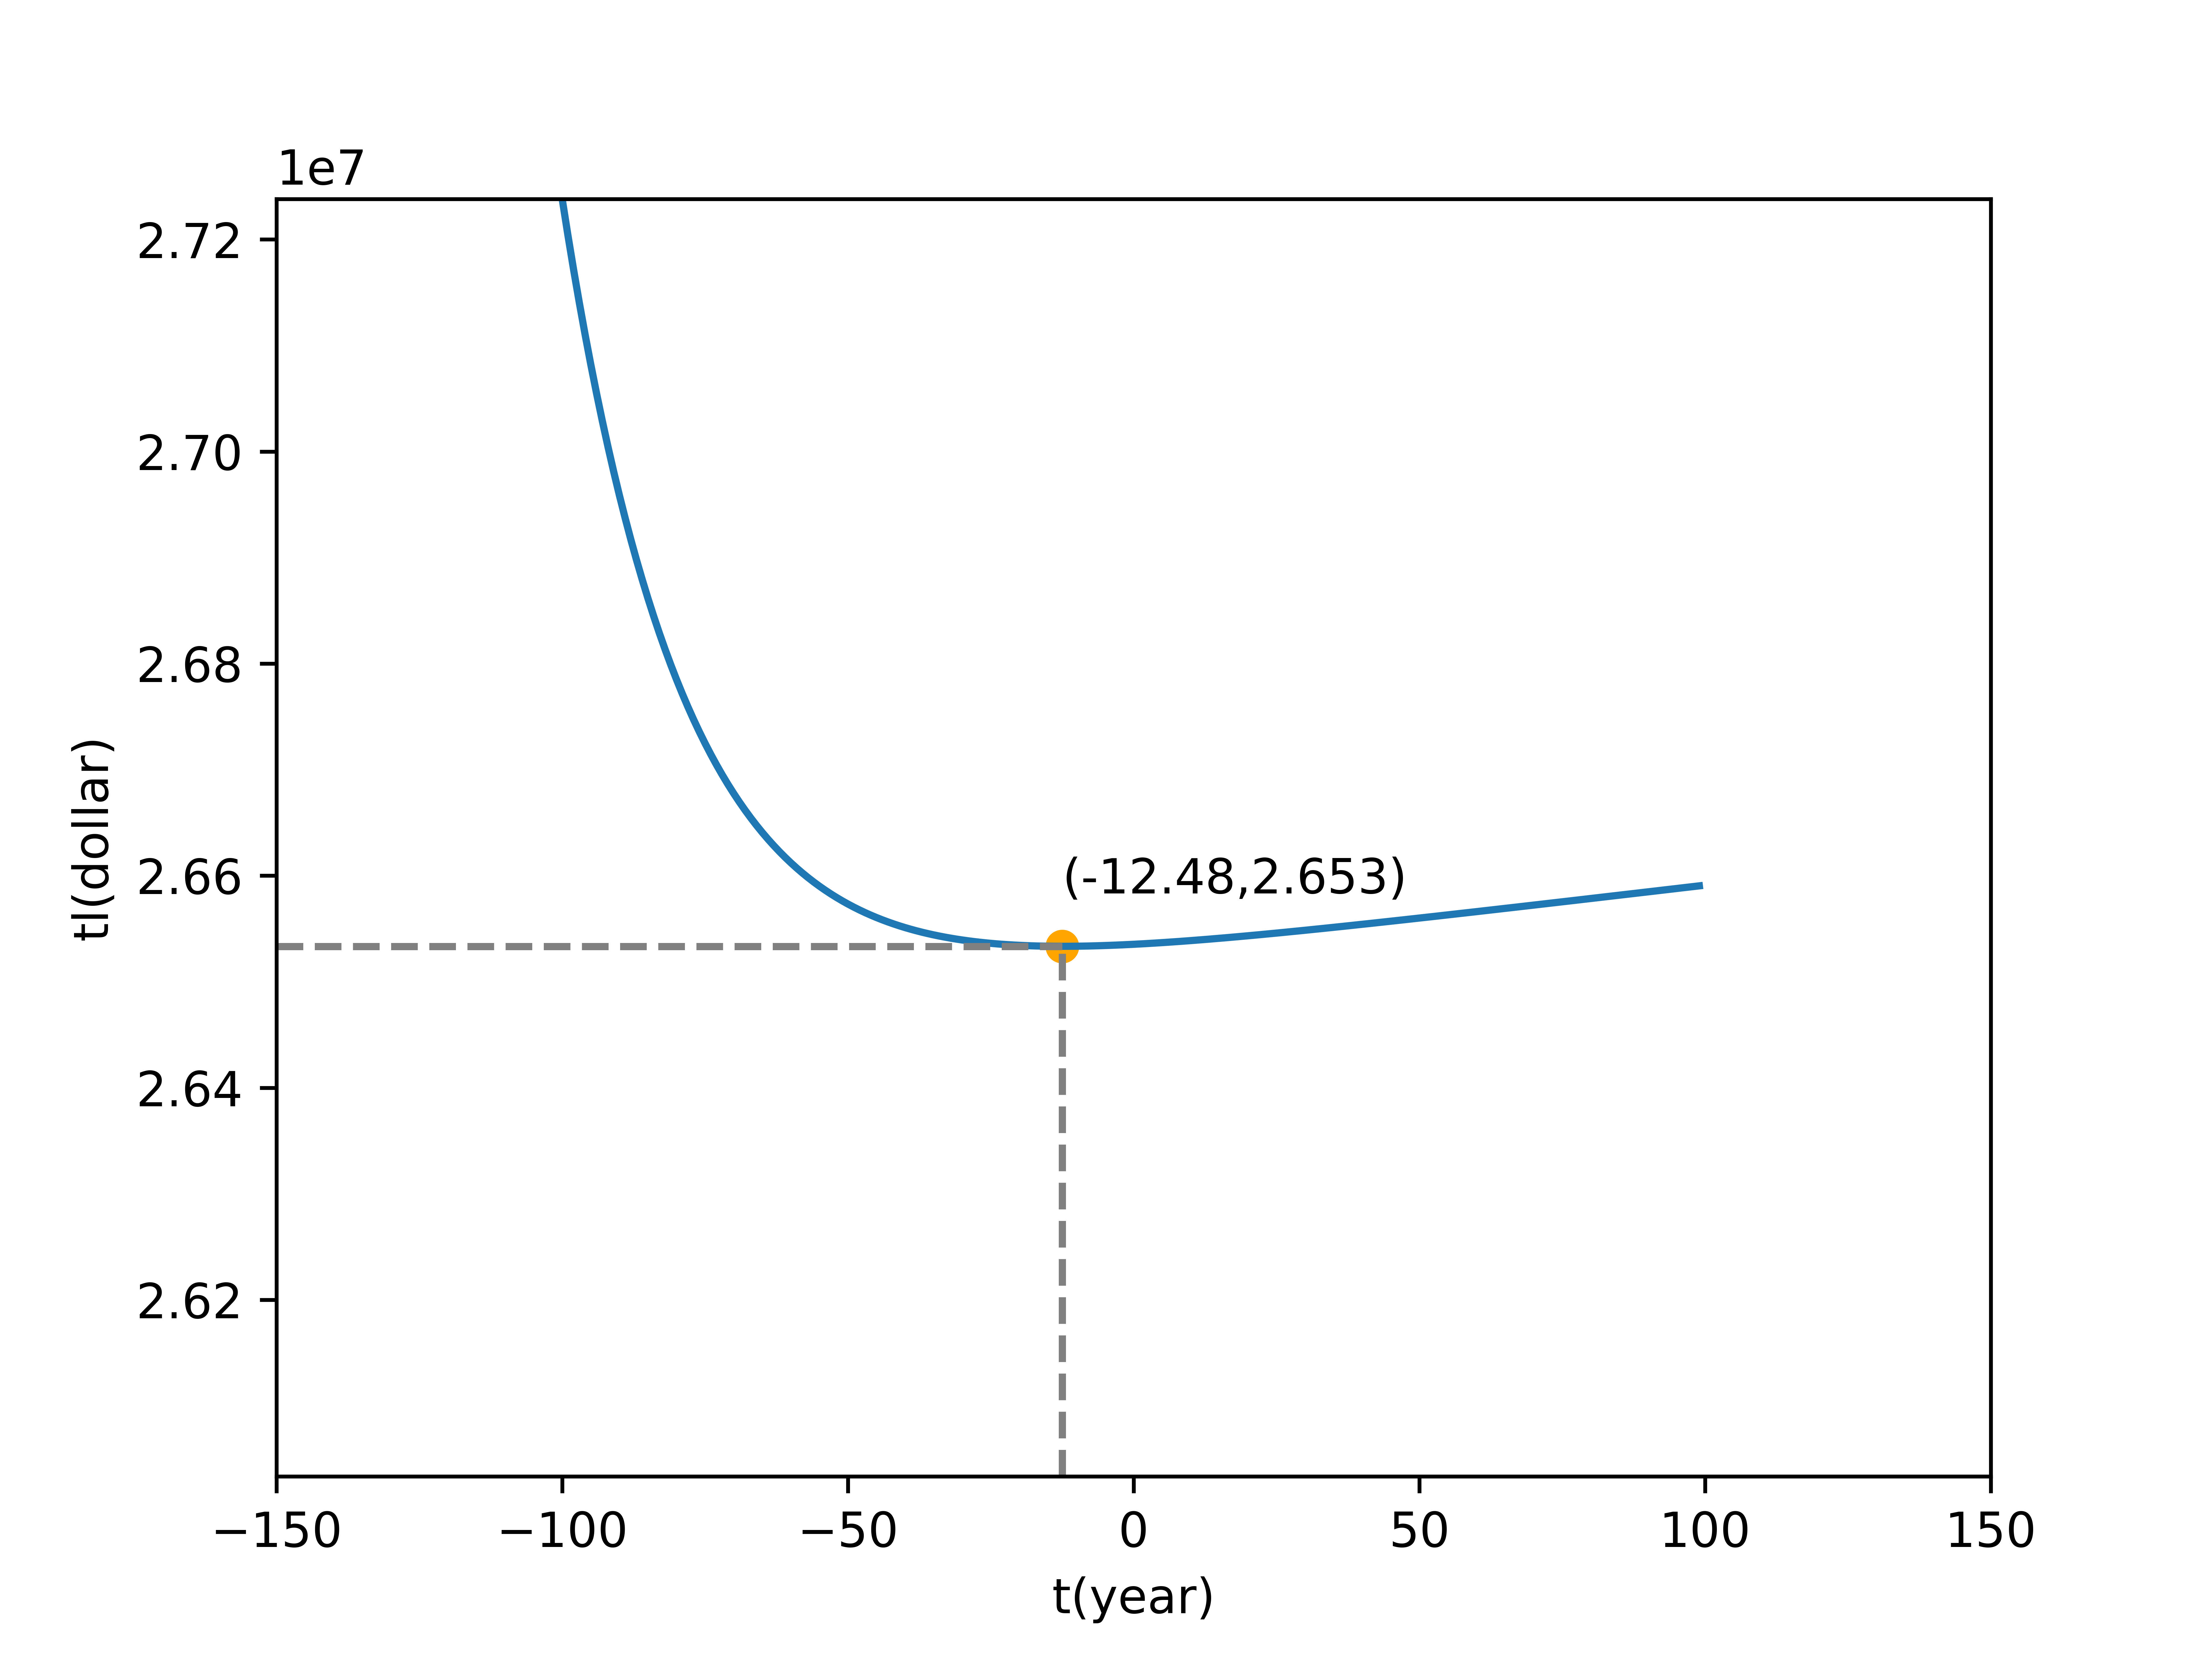
\includegraphics[width=.7\textwidth]{img/img06.png}
\caption{Plot of Migration Time-Cost Function}
\end{figure}

So we conclude that for the next 20 years, Willis Tower will not be relocated, but maintained. The total cost of maintenance is estimated to be 
\begin{align*}
    tl=20 \cdot tv \cdot lpr = 126820
\end{align*}


\section{Strengths and Weaknesses}

\subsection{Model for Predicting the Number of Natural Disasters}
\textbf{Strengths of this model}
\begin{itemize}
    \item Serial correlation has been taken into account and time series analysis has been applied to enhance the resilience of the model. Both the lag of the impact of climate change on natural disasters is shown, while the model will be analyzed on a rolling basis every year. The latest situation of climate change will be taken into account in a timely manner. The model is sensitive to changes in climate change and natural disasters.
    \item The original data of the model includes the number of disasters in each state of the U.S. from 1950 to 2023 on a daily scale. The original data of the model has a large span, and the fitting effect is good. The model is highly interpretive and generalizable.
\end{itemize}

\textbf{Weaknesses of this model}
\begin{itemize}
    \item Considering the complexity of the model, the time series order was chosen to be the same for all regions. Therefore, it cannot accurately reflect the impact of the climate characteristics of each region or the uniqueness of climate change on the number of local disasters.
 \end{itemize}
 
\subsection{Natural Disaster Count-Property Loss Fitting Model}
\textbf{Strengths of this model}
\begin{itemize}
    \item Considering the number of natural disasters and the distributional characteristics of property damage, a nonlinear regression method was selected to build the model. The model was fitted with high goodness of fit.
    \item GDP data for each state for each calendar year was investigated and the stock of assets for each year was calculated using the NASDAQ-100 index for each calendar year as the return on assets. Projections were also fitted to the asset stock. Loss ratios calculated from asset stocks and property losses are more reasonable.
\end{itemize}

\textbf{Weaknesses of this model}
\begin{itemize}
    \item Considering the complexity of the model, only the annual average return on assets was used in the calculation of the return on assets. The accuracy of forecasting the stock of assets for each year is reduced.
 \end{itemize}

\subsection{Underwriting Strategy Model}
\textbf{Strengths of this model}
\begin{itemize}
    \item Using asset pricing theory to strictly determine the optimal underwriting strategy: Assuming the CRRA utility function, so that the heterogeneity of users in terms of property size and risk preferences is fully explained by theta, the relative risk aversion coefficient, and at the same time describes the underwriting strategy as "the process of determining the proportion of the premiums in the various states".
    \item Assuming that insurers only have access to the distribution of theta, and $\theta_i$ of each customer is only known to the customer itself, which is suitable for the information game between the customer and the insurer in the transaction.
    \item Provide an observation method for theta distribution of non-intuitive data: the quartile of the critical $\theta_{bound,j}$ in the overall distribution is derived from the percentage of insured amount in different states, so the mean and variance of theta can be fitted.
    \item Design the evaluation function $Esti$, which translates the business objectives of the insurance company into a requirement for a stochastic distribution of profits
\end{itemize}

\textbf{Weaknesses of this model}
\begin{itemize}
    \item Only consider the underwriting strategy in the monopoly pricing situation.
    \item Not considering the different loss distributions of different types of property under different types of extreme weather.
 \end{itemize}

\subsection{Community and Real Estate Site Selection Model}
\textbf{Strengths of this model}
\begin{itemize}
    \item The modeling process uses the regional price parity (RPP) method to take into account the impact of different price levels in different regions on housing prices and consumption indices, and price level parity processing, so that housing prices and consumption indices can truly reflect the level of housing prices in a region as well as the ability to consume. More accurate estimation of real estate development status and prospects. Make the model more interpretive of the real world.
    \item The final score is not an absolute score, but a relative score after normalization. This makes the model more generalizable and suitable for comparisons between different regions. Real estate companies can decide the development area according to the score ranking situation.
\end{itemize}

\textbf{Weaknesses of this model}
\begin{itemize}
    \item The model only considers the difference between the real estate company and the insurance company's heart price in the scoring pattern. This makes the model less pervasive and can only be applied to situations where there is an insurance option.
 \end{itemize}

\subsection{Architectural Conservation Model}
\textbf{Strengths of this model}
\begin{itemize}
    \item Considering multiple factors or indicators in an integrated manner avoids the limitations of single-factor evaluation, making the evaluation results more comprehensive and objective.
    \item It is applicable to a variety of different types of factors or indicators, including qualitative and quantitative factors, making the method widely applicable.
    \item The evaluation result is a clear value that is easy to understand and apply. This allows decision makers to have a clearer understanding of the overall status of a risk, project or other object, providing strong support for decision making.
\end{itemize}

\textbf{Weaknesses of this model}
\begin{itemize}
    \item The evaluation results depend largely on the subjective judgment of the decision maker. This may lead to a certain degree of subjectivity and uncertainty in the evaluation results, affecting the accuracy and scientificity of decision-making.
 \end{itemize}



\begin{letter}{Letter}
\begin{flushleft}  % 左对齐环境,无首行缩进
\textbf{To:} Government of Chicago\\
\textbf{From:} Team 2411457\\
\textbf{Date:} February 5th, 2024\\
\textbf{Subject:} Recommendations for Future Planning of Chicago's Landmark Willis Tower
\end{flushleft}

Dear Sir/Madam.

The intensification of global climate change in recent years and the increasing frequency and intensity of extreme weather events have been a significant detriment to the development of cities and buildings. In response to this change, we are writing to offer our researched recommendations for the future planning of Chicago's iconic Willis Tower and the City of Chicago.
Globally, the future is characterized by an increase in natural disasters in many areas, as well as an increase in the wear and tear and damage they can inflict on buildings, thus exacerbating the damage.

We first analyzed and predicted the number of natural disasters that may occur in the future, and predicted the future occurrence of natural disasters in various parts of the United States. In the case of Chicago, which is shown on the left side of the graph below, where the horizontal axis is the year and the vertical axis is the number of disasters that occurred, there was no extreme increase in the number of natural disasters. And with the development of science and technology, the damage caused by a single natural disaster will slowly decrease, thus natural disasters will not have an increasing impact on Chicago.

The building preservation model we developed and solved estimates the cost of relocating Chicago's landmark Willis Tower due to environmental concerns in the years following its construction, as shown on the right side of the figure below. The horizontal axis represents the number of years since the building was built, and the vertical axis represents the estimated cost if it were to be relocated at this point. It can be seen that the cost is increasing every year since $t>0$. And the minimum value of the cost is taken at $t=-12.48<0$. Therefore, we get the conclusion that in the next 20 years, there is no need to relocate Willis Tower, but we should pay attention to the maintenance and repair of the building.

\begin{figure}[htbp]
\centering
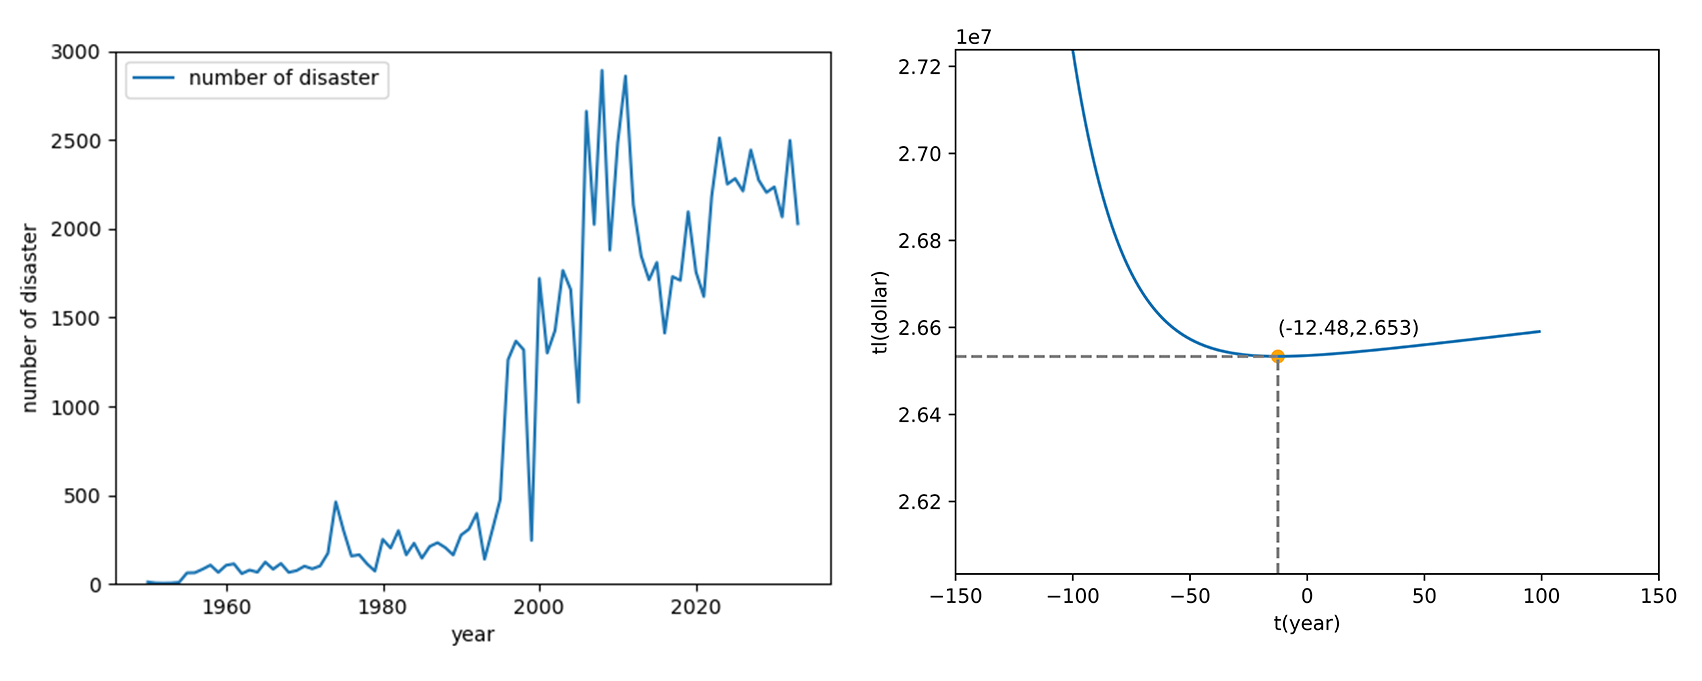
\includegraphics[width=.8\textwidth]{img/img07.png}
\caption{Plot of Migration Time-Cost Function}
\end{figure}

We sincerely hope that the relevant organizations will consider and adopt our suggestions, and hope that the development of the city of Chicago will be steady and good.

Yours Sincerely, Team 2411457

\end{letter}

\newpage

% 参考文献,此处以 MLA 引用格式为例
\begin{thebibliography}{99}

\bibitem{1} Diane P. Horn, Baird Webel. (2023). Private Flood Insurance and the National Flood Insurance Program. Retrive at: \href{https://crsreports.congress.gov}{https://crsreports.congress.gov}

\bibitem{2} Katherine R. H. Wagner. (2021). Adaptation and Adverse Selection in Markets for Natural Disaster Insurance. Retrive at: \href{https://www.krhwagner.com/}{https://www.krhwagner.com/}

\bibitem{3} Kendra Marcoux, Katherine R. H. Wagner. (2023). Fifty Years of U.S. Natural Disaster Insurance Policy. Retrive at: \href{https://www.krhwagner.com/}{https://www.krhwagner.com/}

\bibitem{4} Merton, R. C. (1973). An Intertemporal Capital Asset Pricing Model. Retrive at: \href{https://doi.org/10.2307/1913811}{https://doi.org/10.2307/1913811}

\bibitem{5} L.A. Zadeh. (1965). Fuzzy sets. Retrive at: 
\href{https://www.sciencedirect.com/science/article/pii/S001999586590241X}{https://www.sciencedirect.com/science/article/pii}

\bibitem{6} Laura Bakkensen, Lint Barrage. (2017). Flood Risk Belief Heterogeneity and Coastal Home Price Dynamics: Going Under Water? Retrive at: \href{https://ssrn.com/abstract=3042412}{https://ssrn.com/abstract=3042412}

\bibitem{7} Gallagher, Justin. (2014). Learning about an Infrequent Event: Evidence from Flood Insurance Take-Up in the United States. Retrive at: \href{https://www.doi.org/10.1257/app.6.3.206}{https://www.doi.org/10.1257/app.6.3.206}

\bibitem{8} Markowitz, H. (1952). Portfolio Selection. Retrive at: \href{https://doi.org/10.2307/2975974}{https://doi.org/10.2307/2975974}

\bibitem{9} Fama, E. F., MacBeth, J. D. (1973). Risk, Return, and Equilibrium: Empirical Tests. Retrive at: \href{http://www.jstor.org/stable/1831028}{http://www.jstor.org/stable/1831028}

\bibitem{10} Kapphan, I., Calanca, P., Holzkaemper, A. (2012). Climate Change, Weather Insurance Design and Hedging Effectiveness. Retrive at: \href{http://www.jstor.org/stable/41953179}{http://www.jstor.org/stable/41953179}

\bibitem{11} Cohen, A., Siegelman, P. (2010). Testing for Adverse Selection in Insurance Markets. Retrive at: \href{http://www.jstor.org/stable/20685290}{http://www.jstor.org/stable/20685290}

\bibitem{12} Friedman, H. C. (1971). Real Estate Investment and Portfolio Theory. Retrive at: \href{https://doi.org/10.2307/2329720}{https://doi.org/10.2307/2329720}

\end{thebibliography}

\begin{subappendices}  % 附录环境

\section{Appendix A: Program Codes}
Here are the program codes we used in our research.


% Python 代码示例
\begin{lstlisting}[language=Python, name={var.py}]
# Used for Vectors auto regression(VAR)
import pandas as pd
import numpy as np

combined_forecast_df = pd.DataFrame(index = csv_files)

for index, row in combined_forecast_df.iterrows():
    row_mean = row.mean()
    row_std = row.std()
    combined_forecast_df.loc[index] = np.where(
    combined_forecast_df.loc[index] < 0, 0, 
    combined_forecast_df.loc[index])
    combined_forecast_df.loc[index] = np.where(
    combined_forecast_df.loc[index] > (row_mean + 3 * row_std),
    row_mean + 3 * row_std, combined_forecast_df.loc[index])
    combined_forecast_df.to_csv(output_file)
\end{lstlisting}

\begin{lstlisting}[language=Python, name={cal_theta.py}]
# Used for calculating distribution of theta
# omit import

df = pd.read_excel('ln(lgr).xlsx')
pi_j_lis = [random.uniform(0, 1) for _ in range(50)]
theta_boundj = []
for index, row in df.iterrows():
    result = 2 * pi_j_lis[index] * np.exp(-2 * row['a']) 
    * (1 / (np.exp(2 * row['b^2']) - np.exp(row['b^2'])))
    theta_boundj.append(result)
def f(x):
    return norm.pdf(x)
def F(x):
    return norm.cdf(x)
def func(params, x):
    theta, sigma = params
    return F((x - theta) / sigma) * x / sigma * f((x - theta) / sigma)

x = np.array(theta_boundj)
def loss(params):
    y_pred = np.array([func(params, xi) for xi in x])
    return np.mean(y_pred**2)
init_params = np.array([0.5, 0.5])
result = minimize(loss, init_params, method='SLSQP')
best_params = result.x
\end{lstlisting}

\clearpage

\end{subappendices}  % 附录内容结束

\begin{ReportAiUse}{9}
\bibitem{AI1}
Kimi Chat  \\
Query1: Risk, Return, and Equilibrium: Empirical Tests Find literature related to this article  \\
Output:  Risk, Return, and Equilibrium: Empirical Tests Find literature related to this article.

"Risk, Return, and Equilibrium: Empirical Tests" is a classic paper published by Eugene F. Fama and James D. MacBeth in the Journal of Political Economy in 1973. This paper proposes the famous Fama MacBeth regression method for predicting asset returns. Here are some highly relevant literature related to this article:

Sharpe, W. F. (1964) Capital asset prices: A theory of market equity under conditions of risk The Journal of Finance, 19 (3), 425-442

This paper proposes the Capital Asset Pricing Model (CAPM), which is the cornerstone of modern financial theory and closely related to the Fama MacBeth method in the field of asset pricing.

Fama, E. F.,French, K. R. (1993) Common risk factors in the returns on stocks and bonds Journal of Financial Economics, 33 (1), 3-56

Fama and French proposed a three factor model in this paper, which is an extension of CAPM and has direct application with Fama MacBeth method in empirical asset pricing research.

Fama, E. F.,French, K. R. (2015) A five factor asset pricing model Journal of Financial Economics, 116 (1), 1-22

In this subsequent study, Fama and French further developed their model and proposed a five factor model, which is also an empirical study based on the Fama MacBeth method.


\bibitem{AI2}
WeTab AI Pro \\
Query1: Write an example of using sco.optimize least squares with two variables to obtain results \\
Output: When using scipy. optimize for least squares fitting, you need to define an objective function (also known as a loss function) that takes input from the parameters and variables to be fitted, and returns a measure of the difference between the fitted value and the observed value.

Here is an example of using scipy.optimize for least squares fitting:
\begin{lstlisting}[language=Python]
import numpy as np
from scipy.optimize import least_squares

# Define the function to be fitted
def func(params, x):
    a, b = params
    return a * x + b

# Defining Observations
x = np.array([1, 2, 3, 4, 5])
y_observed = np.array([4.8, 8.5, 10.3, 13.8, 17.2])

# Define objective function (loss function)
def objective(params, x, y_observed):
    return func(params, x) - y_observed

# Initial value of initialization parameters
initial_params = [1, 1]

# Fitting using the least squares method
result = least_squares(objective, initial_params, 
args=(x, y_observed))

# Obtain fitted parameters
a_opt, b_opt = result.x

print("Fitting results:")
print(f"a: {a_opt}")
print(f"b: {b_opt}")
\end{lstlisting}


\end{ReportAiUse}

\end{document}  % 结束
